%%%%%%%%%%%%%%%%%%%%%%%%%%%%%%%%%%%%%%%%%%%%%%%%%%%%%%%%%%%%%%%%%%%%%%%%%%%%%%%
%                         File: osa-revtex4-1.tex                             %
%                        Date: April 15, 2013                                 %
%                                                                             %
%                              BETA VERSION!                                  %
%                   JOSA A, JOSA B, Applied Optics, Optics Letters            %
%                                                                             %
%            This file requires the substyle file osajnl4-1.rtx,              %
%                   running under REVTeX 4.1 and LaTeX 2e                     %
%                                                                             %
%                   USE THE FOLLOWING REVTeX 4-1 OPTIONS:                     %
% \documentclass[osajnl,twocolumn,showpacs,superscriptaddress,10pt]{revtex4-1}%
%                    %% Use 11pt for Applied Optics                           %
%                                                                             %
%               (c) 2013 The Optical Society of America                       %
%                                                                             %
%%%%%%%%%%%%%%%%%%%%%%%%%%%%%%%%%%%%%%%%%%%%%%%%%%%%%%%%%%%%%%%%%%%%%%%%%%%%%%%

\documentclass[osajnl,twocolumn,showpacs,superscriptaddress,10pt]{revtex4-1} %% use 10pt for Applied Optics
%%\documentclass[osajnl,preprint,showpacs,superscriptaddress,12pt]{revtex4-1} %% use 12pt for preprint option
\usepackage{amsmath,amssymb,graphicx,float,enumerate}
\usepackage[cache=false]{minted}
\usepackage[utf8]{inputenc}
\graphicspath{ {../images/} }

\usepackage[colorlinks = true,
            linkcolor = black,
            urlcolor  = blue,
            citecolor = black,
            anchorcolor = blue]{hyperref}

\usepackage{silence}
\WarningFilter{revtex4-1}{Repair the float}

\begin{document}

\title{Redes y Comunicaciones}

\author{Ulises Jeremias Cornejo Fandos}
\affiliation{13566/7, Licenciatura en Informatica, Facultad de Informatica, UNLP}

\author{Federico Ramón Gasquez}
\affiliation{13598/6, Licenciatura en Informatica, Facultad de Informatica, UNLP}

\author{Lihuel Pablo Amoroso}
\affiliation{13497/2, Analista Programador Universitario, Facultad de Informatica, UNLP}

%%\begin{abstract}
%%\end{abstract}

\maketitle %% required

\onecolumngrid

\section{Ejercicio 1}

\textit{Utilizando topología topologia-IP.imn y dado el bloque IPv6: 2001:db8:1234::/48.}

\begin{enumerate}[a)]
    \item Arme el plan de direccionamiento IPv6 teniendo en cuenta las siguientes restricciones:
    
    \begin{itemize}
        \item La red A tiene 70 hosts y se espera un crecimiento máximo de 20 hosts.
        \item La red X tiene 150 hosts.
        \item La red B cuenta con 20 hosts
        \item La red Y tiene 35 hosts y se espera un crecimiento máximo de 30 hosts.
        \item Los bloques IP asignados en los enlaces entre routers podrán ajustarse a desperdiciar pocas direcciones.
        \item Es importante utilizar VLSM?
        
        Para armar el plan de direccionamiento IPv6 de esta topologia no es necesario utilizar VLSM dado que
        la cantidad de host a asignar por red nunca llegan a ser tantas como para que no alcanse la cantidad
        de IPs asignables.
    \end{itemize}

    \item Asigne direcciones IP en los equipos de la topología según el plan anterior.
    
    \item Configure las tablas de rutas teniendo en cuenta las siguientes restricciones:
    
    \item n1 deberá optar por el enlace verde solamente para rutear el tráfico dirigido a la Red X.
    
    \item Utilizando la herramienta ping6(8), verifique conectividad entre los hosts pertenecientes  a las diferentes redes de usuarios.
    

\end{enumerate}

\section{Ejercicio 2}

\textit{TTL (Adjunte capturas de tráfico para cada uno de los incisos).}

\begin{enumerate}[a)]
    \item \textit{Utilizando el comando \textbf{traceroute6/tracepath6(8)}, realice una
    traza entre el host n8 y n10, tanto utilizando UDP como ICMP.
    ¿Qué diferencias tiene cada método y en qué casos utilizaría cada
    uno?.}


    \item \textit{Realice un ping entre n8 y n5 y determine el valor inicial del
    campo TTL capturando tráfico en la interfaz eth0 del host n8.}

    Para este inciso, se ejecuta en la terminal correspondiente al host n8 un ping entre este host y n7
    utilizando el comando \textit{ping6}. \\

    Capturando el tráfico con el wireshark se busca determinar el valor del campo TTL en
    el header del paquete IPv6. Tras no poder encontrarlo se inspecciona el formato de una
    cabecera IPv6 y concluyendo que dicha información se puede obtener en el header Hop Limit. 
    Leer \href{https://tools.ietf.org/html/rfc2460}{RFC 2460}. \\

    Se puede observar entonces en la figura \ref{image:ttl}, que el valor inicial
    del campo TTL, \textit{Hop Limit en IPv6}, es 64.

    \begin{figure}[H]
        \centering
        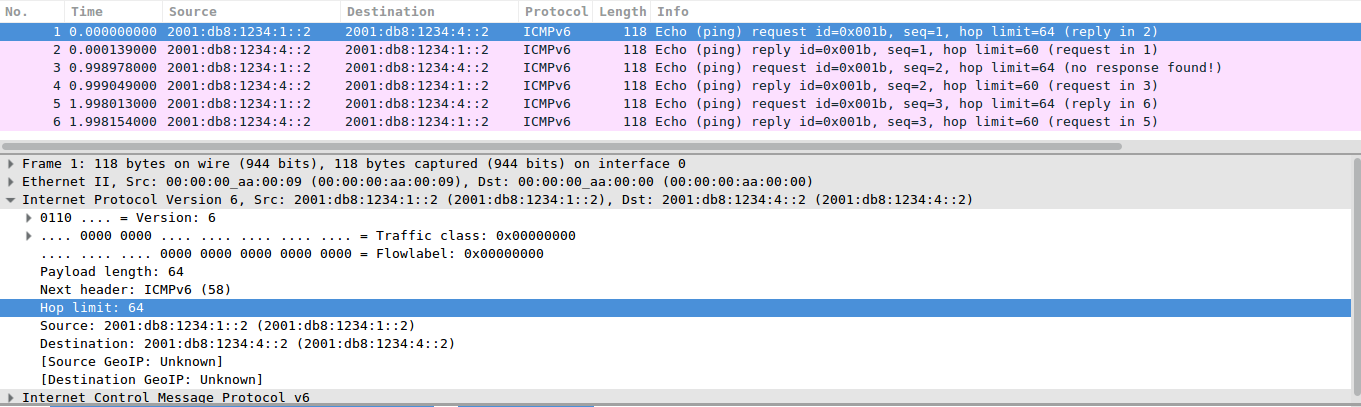
\includegraphics[width=0.95\textwidth]{ttl.png}
        \caption{Captura del tráfico del ping entre n8 y n7 en el que se observa el valor inicial del campo Hop Limit.}
        \label{image:ttl}
    \end{figure}

    \item \textit{A través de la capturas de tráfico, determine en qué momento el
    router decrementa el valor del TTL.}

    

    \item \textit{Utilizando la herramienta para enviar mensajes ICMP con la opción
    -t desde n8 envíe un datagrama a n7 con TTL=1. ¿Qué mensaje recibe? ¿Por qué?}

    Para enviar mensajes ICMP se utiliza el comando ping(6) ejecutando, en la 
    terminal del nodo n8, el siguiente comando,

    \begin{minted}{bash}
    $ ping6 -t 2001:db8:1234:4::2
    \end{minted}

    siendo 2001:db8:1234:4::2 la IPv6 del nodo n7. \\

    A la par que se envía el datagrama, se captura el tráfico utilizando wireshark
    como se observa en la figura (\ref{image:ttl1}). El mensaje que se recibe tanto en la
    salida del comando ejecutado (figura \ref{image:ttl1ping}) como en los paquetes
    capturados por el wireshark es \textit{Time exceeded: Hop Limit}.

    \textbf{TERMINARRRRRRRRR}

    \begin{figure}[H]
        \centering
        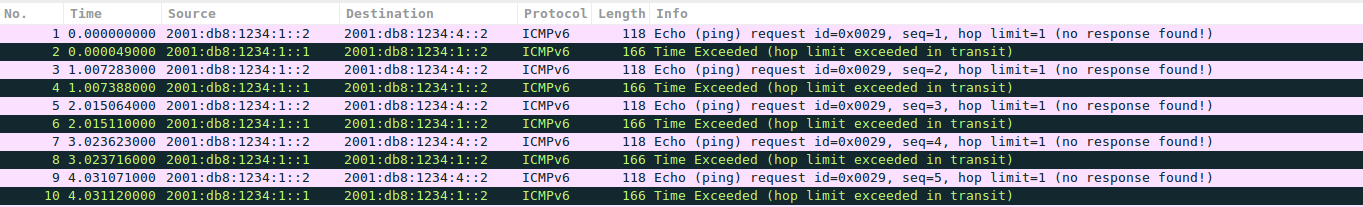
\includegraphics[width=0.95\textwidth]{ttl1.png}
        \caption{Captura del tráfico del ping entre n8 y n7.}
        \label{image:ttl1}
    \end{figure}

    \begin{figure}[H]
        \centering
        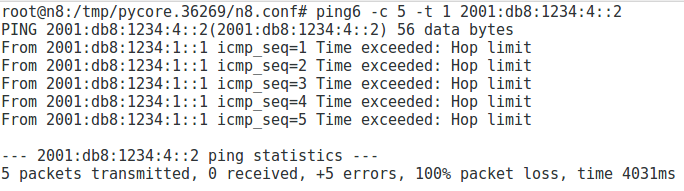
\includegraphics[width=0.75\textwidth]{ttl1ping.png}
        \caption{Salida del comando ping.}
        \label{image:ttl1ping}
    \end{figure}
\end{enumerate}

\section{Ejercicio 3}

\textit{Dual Stack}

\begin{enumerate}[a)]
    \item Configure en la parte “X” y en “B” la red en IPv4 e IPv6 en modo Dual Stack.
    
    \item Genere tráfico IPv6 e IPv4 y compare.
    
    \item Investigue mecanismos para llevar el tráfico IPv4 de la red “X” a la red “B” pasando por redes. Vea cómo puede implementarse en la topología.

\end{enumerate}

\end{document}
